\documentclass[letterpaper,12pt,fleqn]{article}
\usepackage{matharticle}
\pagestyle{empty}
\newcommand{\cycle}[1]{\left<#1\right>}
\newcommand{\n}{\mathrel{\triangleleft}}
\begin{document}
\section*{Free Abelian Groups}

\begin{definition}
  Let $G$ be an abelian group and $X\subseteq G$. To say that $X$ is a basis
  for $G$ means:
  \begin{enumerate}
  \item $G=\cycle{X}$
  \item $\forall\,x_k\in X$ distinct and $n_k\in\N$:
    \[\sum_{k=1}^nn_kx_k=0\iff\forall\,n_k=0\]
  \end{enumerate}
\end{definition}

\begin{example}
  $G=\bigoplus_{i=1}^nZ$

  Let $x_k=\begin{cases}
  1, i=k \\
  0, i\ne k
  \end{cases}$
\end{example}

\begin{theorem}
  Let $F$ be an abelian group. TFAE:
  \begin{enumerate}
  \item $F$ has a non-empty basis.
  \item $F$ is the internal direct sum of a family of infinite cyclic groups.
  \item $F$ is isomorphic to a direct sum of copies of $\Z$.
  \item There exists a non-empty set $X$ and function $\iota:X\to F$ such that
    given an abelian group $G$ and a function $f:X\to G$, there exists a
    unique homomorphism $\phi:F\to G$ such that $f=\phi\iota$.
  \end{enumerate}

  \begin{figure}[h]
    \setlength{\leftskip}{1in}
    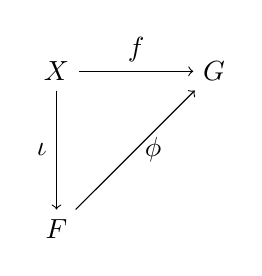
\begin{tikzpicture}
      \node (X) at (0,2) {$X$};
      \node (G) at (2,2) {$G$};
      \node (F) at (0,0) {$F$};
      \draw [->] (X) to node [above] {$f$} (G);
      \draw [->] (X) to node [left] {$\iota$} (F);
      \draw [->] (F) to node [right] {$\phi$} (G);
    \end{tikzpicture}
  \end{figure}

  A group $F$ that satisfies these properties is called a \emph{free} abelian
  group.
\end{theorem}

\begin{theproof}
  \listbreak
  \begin{description}
  \item $1\to 2$: Assume $F$ has a non-empty basis $X$

    Assume $x\in X$ \\
    $nx=0\implies n=0$ \\
    Thus, $\cycle{x}$ is infinite cyclic \\
    Since $F$ is abelian, $\cycle{x}\n F$ \\
    Since $X$ is a basis, there exists a set $\{x_k\}\subseteq X$ such that
    $F=\cycle{\bigcup_{k=1}^n\cycle{x_k}}$ \\
    Assume $z\in X$ \\
    ABC: $\cycle{z}\cap\cycle{\bigcup_{x_k\ne z}\cycle{x_k}}\ne\{0\}$ \\
    $\exists\,n\in\N,nz=\sum_{k=1}^n{n_kx_k}$ \\
    $nz+\sum_{k=1}^n{n_kx_k}=0$; however, $n\ne0$ \\
    Contradiction (of basis)! \\
    So $\cycle{z}\cap\cycle{\bigcup_{x_k\ne z}\cycle{x_k}}=\{0\}$ \\
    $\therefore F$ is an internal direct sum of the $\cycle{x_k}$.

  \item $2\to 3$: Assume $F$ is the internal direct sum of a family of
    infinite cyclic groups

    Let $F=\sum F_k$ be such a sum \\
    $F\simeq\bigoplus F_k$ \\
    $F_k\simeq Z$ \\
    There exists an isomorphism $\phi_k:F_k\to Z$ \\
    Therefore there exists an isomorphism $\phi:F\to\bigoplus\Z$.

  \item $3\to 1$ Assume $F$ is isomorphic to a direct sum of copies of $\Z$

    Let $\{u_k\}$ be the standard basis for $\bigoplus\Z$ \\
    There exists isomorphism $\phi:\bigoplus\Z\to F$ \\
    Let $x_k=\phi_k(u_k)$ \\
    Let $X=\{x_k\}$ \\
    Let $f_i=\phi(z_i)$ \\
    $f_i=\phi(\sum n_ku_k)=\sum\phi_k(n_ku_k)=\sum n_k\phi_k(u_k)=\sum n_kx_x$ \\
    Thus, $F=\cycle{X}$

    Now, assume $\sum n_kx_k=0$ \\
    $\phi^{-1}(\sum n_kx_k)=\sum\phi_k^{-1}(n_kx_k)=\sum n_k\phi^{-1}(x_k)=
    \sum n_ku_k=0$ \\
    This, $\forall\,n_k=0$

    Therefore, $X$ is a basis for $F$.

  \item $1\to 4$: Assume $F$ has a non-empty basis $X$

    Let $\iota:X\to F$ be the canonical injection homomorphism

    Assume $G$ is an abelian group and $f:F\to G$ \\
    Assume $u\in F$ \\
    $u=\sum_{k=1}^nn_kx_k$ \\
    Assume $u=\sum_{k=1}^nm_kx_k$ \\
    $\sum_{k=1}^nn_kx_k-\sum_{k=1}^nm_kx_k=\sum_{k=1}^n(n_k-m_k)x_k=0$ \\
    But $n_k-m_k=0$ since $X$ is a basis for $F$ \\
    So the representation for each $u\in F$ is unique wrt basis $X$

    Let $\phi:F\to G$ be defined by $\phi(u)=\phi(\sum_{k=1}^nn_kx_k)=
    \sum_{k=1}^nn_kf(x_k)$ \\
    Since the representation for each $u\in F$ is unique, $\phi$ is
    well-defined

    Assume $u,v\in F$
    \begin{eqnarray*}
      \phi(u+v) &=& \phi(\sum_{k=1}^nn_kx_k+\sum_{j=1}^nm_jx_j) \\
      &=& \phi(\sum_{k=1}^n(n_k+m_k)x_k) \\
      &=& \sum_{k=1}^n(n_k+m_k)f(x_k) \\
      &=& \sum_{k=1}^nn_kf(x_k)+\sum_{k=1}^nm_kf(x_k) \\
      &=& \phi(u)+\phi(v)
    \end{eqnarray*}
    Therefore $\phi$ is a homomorphism

    Assume that there is another such homomorphism $\psi$ \\
    Since $X$ generates $F$ \\
    So the action of $\psi$ on $F$ is completely determined by $\psi$ on $X$ \\
    Assume $x\in X$ \\
    $\psi(x)=\psi(\iota(x))=(\psi\iota)(x)=f(x)=(\phi\iota)(x)=\phi(\iota(x))=
    \phi(x)$

    \item $4\to 3$ 
  \end{description}
\end{theproof}

\end{document}
